\documentclass[12pt]{amsart}
%\documentclass{amsart}
\usepackage[utf8]{inputenc}
\usepackage{graphicx}
\usepackage{amssymb}
\usepackage{amsmath}
\usepackage{epstopdf}
\usepackage{amsthm}
\usepackage{xypic}
\usepackage{enumerate}
%\usepackage{sidenotes}

%\usepackage{fourier}
%\usepackage{a4wide}


\newtheorem{definition}{Definition} 
\newtheorem{proposition}[definition]{Proposition} 
\newtheorem{theorem}[definition]{Theorem} 
\newtheorem{lemma}[definition]{Lemma} 
\newtheorem{corollary}[definition]{Corollary}
\newtheorem{conjecture}[definition]{Conjecture}
\newtheorem{question}[definition]{Question}
\newtheorem{claim}[definition]{Claim}
\newtheorem{fact}[definition]{Fact}
\newtheorem{remark}[definition]{Remark}
\newtheorem{wedgelemma}[definition]{Wedge Lemma} 
\newtheorem{construction}[definition]{Construction}
\newtheorem{example}[definition]{Example}


\newcommand{\lo}{\preceq}
\newcommand{\rar}{\rightarrow}
\newcommand{\rAr}{\Rightarrow}
\newcommand{\lrAr}{\Leftrightarrow}
\newcommand{\RR}{\mathbb{R}}
\newcommand{\NN}{\mathbb{N}}
\newcommand{\QQ}{\mathbb{Q}}
\newcommand{\ZZ}{\mathbb{Z}}
\newcommand{\HHH}{\mathcal{H}}
\newcommand{\AAA}{\mathcal{A}}
\newcommand{\SSS}{\mathcal{S}}
\newcommand{\FFF}{\mathcal{F}}
\newcommand{\K}{\mathbf{K}}
\renewcommand{\L}{\mathbf{L}}
\newcommand{\U}{\mathbf{U}}
\newcommand{\V}{\mathbf{V}}
\newcommand{\X}{\mathbf{X}}
\newcommand{\Rat}{\operatorname{Rat}}
\newcommand{\ehr}{\operatorname{ehr}}
\newcommand{\dist}{\mathsf{dist}}
\newcommand{\sgn}{\mathrm{sgn}}
\newcommand{\sprod}[2]{\langle #1, #2 \rangle}
\newcommand{\mspan}{\operatorname{span}}
\renewcommand{\dim}{\mathsf{dim}\ }
\newcommand{\inter}{\mathsf{int}\ }
\newcommand{\median}{\mathrm{median}\ }
\DeclareMathOperator*{\argmin}{arg\,min}

\newcommand{\defn}[1]{\emph{#1}}
\newcommand{\norm}[1]{|| #1 ||}

\newcommand{\Glat}{G^{\operatorname{lat}}}
\newcommand{\Gdep}{G^{\operatorname{dep}}}
\newcommand{\Gfine}{G^{\operatorname{fine}}}
\newcommand{\Gfinem}{G^{\operatorname{fine*}}}

\newcommand{\FD}{\mathcal{F}}

\newcommand{\path}{\operatorname{path}}
\newcommand{\reldep}[2]{{#1} \longrightarrow {#2}}
\newcommand{\reldepi}[3]{{#1} \overset{#2}{\longrightarrow} {#3}}
\newcommand{\shift}[2]{\rightarrow(#1,{#2})}
\newcommand{\shiftw}[3]{\overset{#1 \cdot #2}{\longrightarrow} {#3}}

\newcommand{\conv}{\operatorname{conv}}
\newcommand{\cone}{\operatorname{cone}}
\newcommand{\lev}{\operatorname{lev}}
\newcommand{\Lev}{\operatorname{Lev}}
\renewcommand{\deg}{\operatorname{deg}}
\renewcommand{\dim}{\operatorname{dim}}
\renewcommand{\min}{\operatorname{min}}
\renewcommand{\max}{\operatorname{max}}
\newcommand{\fract}{\operatorname{frac}}
\newcommand{\integ}{\operatorname{int}}
\newcommand{\relint}{\operatorname{relint}}

\newcommand{\twin}{\mathsf{twin}}
\newcommand{\hull}{\mathsf{hull}}
\newcommand{\diam}{\mathsf{diam}}
\newcommand{\choice}[1]{\left\{ \begin{array}{ll} #1 \end{array} \right.}
\newcommand{\floor}[1]{\lfloor {#1} \rfloor}
\newcommand{\ceil}[1]{\lceil {#1} \rceil}
\newcommand{\mset}[2]{ \left\{ #1 \; \middle| \; #2 \right\}}
\newcommand{\lk}{\mathsf{lk}}
\newcommand{\sd}{\mathsf{sd}}
\newcommand{\Pa}{\mathrm{P}}
\newcommand{\dotcup}{\ensuremath{\mathaccent\cdot\cup}}
\newcommand{\Hom}{\mathrm{ Hom}}

\begin{document}
\title{Scheduling Problems}
\author{Felix Breuer, Caroline J. Klivans}



\begin{abstract}{(Placeholder basically from my talk abstract) We introduce new families of polynomials associated to scheduling problems.  Our starting point is the consideration of counting functions which enumerate the number of solutions to certain scheduling problems.  These scheduling problems arise naturally in the context of the normal fan of a related polytope.  This approach creates a connection to Erhart theory and quasisymmetric functions which allows us to establish polynomiality of the counting functions easily. Moreover, from these perspectives we establish bounds on the coeffiecients of the polynomials, reciprocity theorems and nonnegativity of certain basis exapansions. 

This approach includes certain classic polynomials arising in geometric combinatorics such as the chromatic polynomial, but also polynomials that do not satisfy contraction/deletion and hence are not generally Tutte invariants.  For example, we define the arboricity polynomial which counts the number of matroid covers with a fixed number of independent sets.}
\end{abstract}
\maketitle


\tableofcontents

%%%%%%%%%%%%%%%%%%%%%%%%%%%%%%%%%
\section{Introduction}
%%%%%%%%%%%%%%%%%%%%%%%%%%%%%%%%%



A \defn{scheduling problem} $S$ on $d$ items is given by a boolean formula $\phi$ over atomic formulas $\omega_i\leq \omega_j$ for $i,j\in[d]$. A \defn{$k$-schedule} solving $S$ is a function $\omega:[n]\rightarrow[k]$ such that $\phi(\omega)$ is true.

* Constraint satisfaction problem.



\section{Motivating examples}

*** Illustrate the overall ideas and methods through a motivating example(s).  Choose examples that are not the 'prettiest', namely that would not fall under other methods, and do not just do the chromatic polynomial. ****

Given a graph, most naturally we consider the graphical arrangement,
the subarrangement of the Braid arrangement given by hyperplanes
indexed by edges in the graph.

Given a matroid, we consider the matroid polytope formed by the convex
hull of the support vectors of bases.  The normal fan of the matroid
polytope is refined by the Braid arrangement, but this fan and the
graphical arrangement are not the same.  

We considered the very special case of graphical matroids.  Matroids
whose bases correspond to spanning trees of a graph.  Take the
\emph{matroid polytope} approach to a graphical matroid.  What integer
points / weight classes / relative orderings are induced?  We saw more
complicated 'rules', for example:\\

$x_1 \neq x_2$ if $x_3 \geq x_1$.  But $x_1 = x_2$ is ok if $x_3 < x_1$.\\

We interpreted this as {\bf{scheduling}} of tasks.  Tasks $x_1$ and
$x_2$ can be performed  at the same time only if $x_3$ happens first.

\begin{figure}[h]
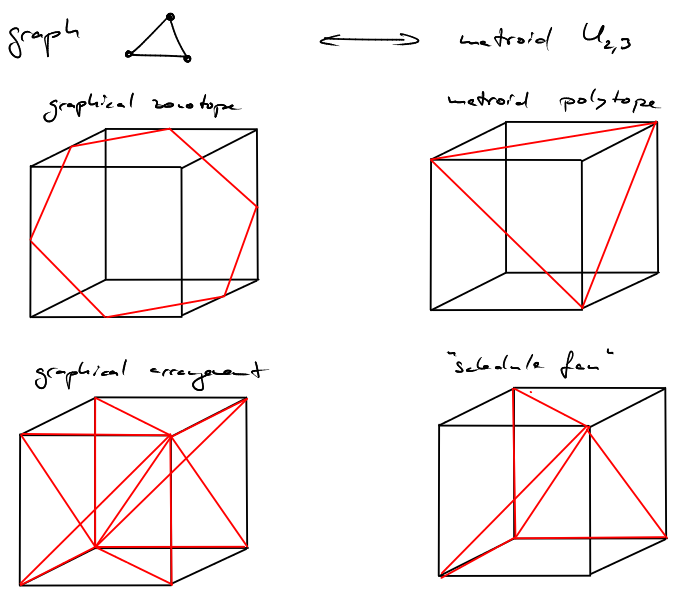
\includegraphics[width=13cm]{graph-matroid}
\caption{Difference between graph construction and graphical matroid construction.}
\end{figure}


\begin{figure}[h]
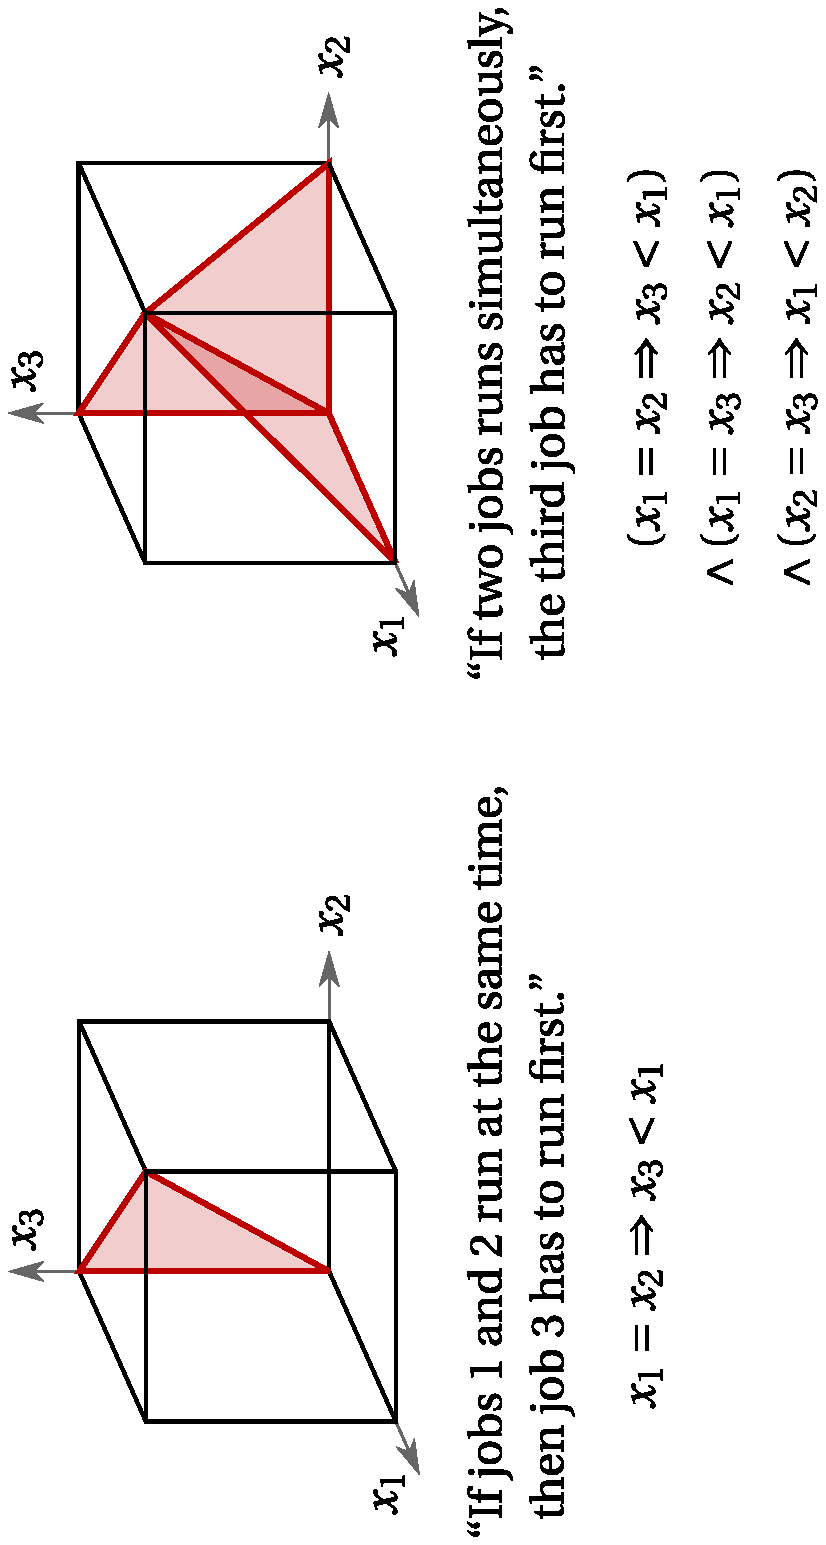
\includegraphics[width=13cm]{schedule}
\caption{Two "scheduling arrangements".}
\end{figure}

** In Figure 2, we should replace implies with AND to keep everything a Boolean formula over pairwise comparisions. 

\section{Preliminaries: Ehrhart Theory}

*** cjk: We will need a Preliminaries: Ehrhart Theory section.  I don't know if it should go before or after the next one.
I have given a minimal introduction to the coxeter complex (of type A), quasisymmetric functions and NCQSym.  Telling a very narrow narrative so as to think about these objects specifically the way we want to use them. ***



\section{Preliminaries: Coxeter Complexes, QSym and NCQsym}

\subsection{Quasisymmetric functions}
A quasisymmetric function is a formal power series in infintely many
variables which has bounded degree and is shift invariant.  Namely for
a composition $\alpha$, the coefficients of all terms
$x_{i_1}^{\alpha_1}x_{i_2}^{\alpha_2} \cdots x_{i_k}^{\alpha_k}$,
running over all possible $k$-tuples $\{i_1, i_2, \ldots, i_k \}$, are
the same.


The monomial quasisymmetric function indexed by the composition $\alpha$ is 
$$M_{\alpha} := \sum_{1 \leq i_1 < i_2 < \ldots < i_k}
x_{i_1}^{\alpha_1} \ldots x_{i_k}^{\alpha_k}.$$  One may equivalently
define quasisymmetric functions as any series which may be written as a
linear combination of monomial quasisymmetric functions, i.e. the
monomial quasisymmetric functions form a basis for the ring of all
quasisymmetric functions.  Clearly any collection of
compositions of $n$ gives rise to a quasisymmetric function simply by
taking the sum of monomial quasisymmetric functions indexed by
compositions in the collection.

** cjk: could include here a discuss of quasisymmetric functions that have
been considered in 'geometric combinatorics', chromatic, matroid,
generalized permutahedra **

\subsection{The Coxeter Complex of Type A}
We want to work at the level of ordered set partitions instead of
compositions.  The correct setting is what is known as 
quasisymmetric functions in non-commuting variables, NCQSym.

Before defining these classes, we motivate working with ordered set
partitions by considering the Coxeter complex of type $A$.  Many of
our arguments will be of a geometric nature concerning the structure
of this complex.


An \emph{ordered set partition} or \emph{set composition} $F \vDash
[n]$ is a sequence of sets $(F^1,F^2, \ldots, F^k)$ such that $\forall
i,j$, $ F^i \cap F^j = \empty$ and $\cup_i F^i = [n]$.  The $F^i$ are the
blocks of the ordered set partition and we will often use the notation
$F^1 | F^2 | \ldots | F^k$.  Note that within each block, elements are
not ordered, so the ordered set partition $13|4|2 \vDash [4]$ is the
same as $31|4|2$.

**fb: Are the $F^i$ allowed to be empty?**


The Braid arrangement $\mathcal{B}_n$ is the hyperplane arrangement in
$\mathbb{R}^n$ consisting of hyperplanes $x_i = x_j$ for all $i,j$.
Note that this arrangement is central, that is all hyperplanes contain
the origin, it is also non-essential, that is the collection of
normals to the hyperplanes do not span all of $\mathbb{R}^n$.  The
hyperplanes have a common intersection equal to the line $x_1 = x_2 = \cdots
= x_n$.  Projecting the arrangement to the orthogonal complement of
this line and intersecting with the unit sphere yields a spherical
simplicial complex known as the \emph{Coxeter complex of type $A$}.
It can be realized combinatorially as the baricentric subdivision of the
boundary of the simplex.


The faces of the Coxeter complex can naturally be labeled by ordered
set partitions.  Each face of the Coxeter complex is simply a
normalization of a face of the cell decomposition induced by
$\mathcal{B}_n$ on $\mathbb{R}^n$.  A face of the cell decomposition specifies for each pair $i,j$ whether $x_i < x_j$, $x_i > x_j$, or $x_i = x_j$.  Namely, all points in a fixed face have
the same relative ordering of coordinates.  This relative ordering
induces an ordered set partition on $[n]$.  For example, if a face
consists of all points such that $x_{i_1} = x_{i_2} < x_{i_3} =
x_{i_4} = x_{i_5} < x_{i_6}$ then the induced ordered set partition is
$12|345|6$.  Under this correspondence, we see that each facet
corresponds to a partition into blocks of size one (i.e. a full
permutation).  Morover, a face $G_1$ is contained in a face $G_2$ iff
the ordered set partition of $G_1$ coarsens the ordered set partition
corresponding to $G_2$.  Hence a collection of ordered set partitions
closed under coarsening gives a subcomplex of the Coxeter complex.

\begin{figure}
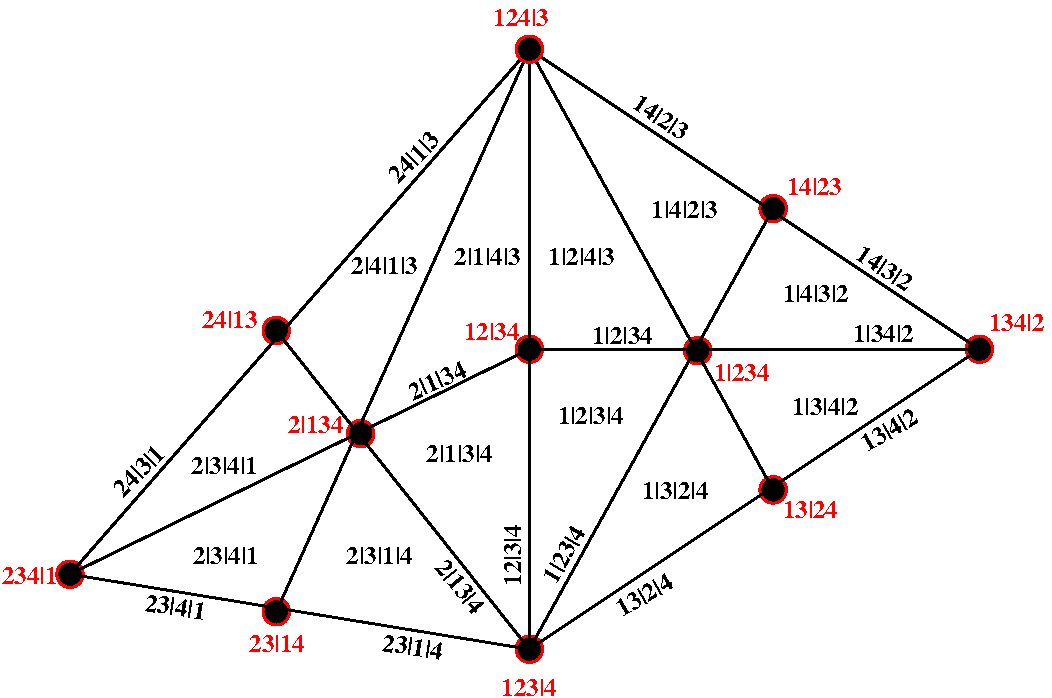
\includegraphics[height=2.5in]{Cox.pdf}
\end{figure}


**Figure of Coxeter complex labeled with ordered set partitions.**

\subsection{Noncommuting Variables}


%% NCSym are symmetric functions indexed by set partitions.  NCQSym are
%% quasisymmetric functions indexed by ordered set partitions, sometimes
%% called set compositions.  (Think of this as analogous to moving from
%% partitions to compositions when one moves from symmetric functions to
%% quasisymmetric functions).


Let $\{x_1, x_2, \ldots \}$ be a collection of non-commuting
variables.  Given $\omega\in \mathbb{R}^n$, let $\mathcal{F}(\omega)$
be the ordered set partition $(F_1,F_2, \ldots F_k)$ such that 
%flag of subsets $\empty = F_0 \subset F_1 \subset \ldots
%\F_{k+1} =[n]$ such that 
$\omega$ is constant on each set $F_i$
%\backslash F_{i-1}$ 
and satisfies $\omega|_{F_i} < \omega|_{F_{i+1}}$ for all $1 \leq i \leq k$. 
%We call $\mathcal{F}(\omega)$ the flag of $\omega$ and
Define the weight class of $\omega$ to be the set of vectors $\nu$
such that $\mathcal{F}(\nu) = \mathcal{F}$.  The weight class $\nu$ consists of all 
points such that the relative size of their components is the same.

\begin{example}
For $\omega = (3,2,2,3,1) \in \mathbb{R}^5$, $\mathcal{F}(\omega) =
(5|23|14)$.  The weight class of $\omega$ consists of all vectors $x
\in \mathbb{R}^5$ such that $x_5 < x_2 = x_3 < x_1 = x_4$. 
\end{example}

Note that
we have again specified the relative ordering of coordinates and a
weight class is simply all points in the relative interior of a cone
of the Braid arrangement and hence naturally associated to a face of
the Coxeter complex.


\begin{definition}
A function in non-commuting variables is called quasisymmetric (an element of NCQsym) if
$\forall \, \gamma, \tau \in \mathbb{N}^n$ such that $\gamma$ and $\tau$
are in the same weight class, $\mathcal{F}(\gamma) =
\mathcal{F}(\tau)$, the coefficient of $x_{\gamma_1}x_{\gamma_2} \cdots
x_{\gamma_n}$ is the same as the coefficient of $x_{\tau_1}x_{\tau_2} \cdots x_{\tau_n}$.
\end{definition}

Let $F$ be an ordered set partition.  Define the monomial quasisymmetric function in non-commuting variables indexed by $F$ as follows:
$$M_F = \sum_{\omega \in \mathbb{N}^n \, \mathcal{F}(\omega) = F} {\bf{x}}_{\omega}$$

Again, one could alternatively define the quasisymmetric functions in
non-commuting variables to be any sum of the monomials.  Most of the
algebra of NCQSym is done at the level of monomials or other bases
indexed by ordered set partitions without reference to the specific
variables.  


\begin{example}

Consider the weight class of  points that satisfy $\omega_1 = \omega_3 < \omega_2 = \omega_4$.  The corresponding ordered set partition $S$ is $(13|24)$.  
$$M_S = x_1x_2x_1x_2 + x_1x_3x_1x_3 + x_2x_3x_2x_3 + x_3x_4x_3x_4 + \cdots$$  

\end{example}

\subsection{From NCQsym to QSym}

As we have seen, elements of QSym are naturally indexed by
compositions and elements of NCQSym are naturally indexed by ordered
set partitions.  We can use the type map from partitions to
compositions to specialize an element of NCQSym to an element of QSym.
The type map of a partition simply records the size of each block.
$$\textrm{type}(B_1|B_2|\cdots|B_n) = (|B_1|, |B_2|, \cdots, |B_n|)$$
If $\mathcal{S} \in NCQSym$ is written as a sum of monomial terms,
applying the type map to each index is equivalent to allowing the
variables to commute.

\begin{example}
Let $\mathcal{S} = M_{(1|23)} + M_{(3|21)} + M_{(2|1|3)}$ be an element of NCQSym written in terms of monomials.  Then 
{type} $\mathcal{S} :=  M_{\textrm{type} (1|23)} + M_{\textrm{type} (3|12)} + M_{\textrm{type} (2|1|3)} = 2 M_{(1,2)} + M_{(1,1,1)}$. Where the right hand side is a quasisymmetric function given in the monomial basis indexed by compositions.  
\end{example}



Given a quasisymmetric function in non-commuting variables (or
commuting), there is also a naturally associated polynomial function
defined by setting the first $m$ variables equal to $1$. 

\begin{example}
Writing ${\bf 1}^m$ for the vector of $1$s of length $m$, and continuing the example above, we have 
$$ \mathcal{S}({\bf 1}^m) = 2 {m \choose 2} + {m \choose 3}$$.  

\end{example}


\section{Scheduling Problems}

Now we have both preliminary sections and should return to scheduling problems.

Define, interpret in both contexts, general theorems.  

*** We also haven't yet talked about hyperplane/polytope duality, generalized permutahedrons, normal fans, the connection to the Braid arrangement.  We can start this section with that material or some of the more general polytope theory can be back in the Erhart section.  For those who would skip a general Erhart section, this is a better place for the material.  It also might make it easier to lead into the technical results.  *****




A \defn{scheduling problem} $S$ on $d$ items is given by a boolean formula $\phi$ over atomic formulas $\omega_i\leq \omega_j$ for $i,j\in[d]$.
 A \defn{$k$-schedule} solving $S$ is a function $\omega:[n]\rightarrow[k]$ such that $\phi(\omega)$ is true. Note that equivalently $\omega$ can also be viewed as a vector $\omega\in [k]^{[n]}$ or as an ordered set partition $\FFF(\omega)$ of $[n]$ into $k$ possibly empty parts. Therefore we will write $\phi(F)$ to mean $\phi(\omega)$ for any $\omega$ such that $\FFF(\omega)=F$ and not that the value of $\phi(F)$ will only depend on $F$ not on the choice of $\omega$. The schedule function $\SSS_S$ in non-commuting variables $x_i$ for $i\in \NN$ is defined as
\[
  \SSS_S = \sum_{\omega\in \NN^n: \phi(\omega) } x_\omega
\] 
The schedule counting function $\xi_S(k)$ is defined as
\[
  \xi_S(k) = \# \text{$k$-schedules $\omega$ such that $\phi(\omega)$ }.
\]


So, geometrically, a satisfiable Scheduling problem can be thought of
as a collection of (relative interiors) of faces of the Coxeter
complex (more correctly, the cell decomposition of space induced by
the Braid arrangement).  This does feel awfully restrictive, it does
not include flow and tension for example as they need (among other
things) the coordinate hyperplanes.  On the other hand, this is a
natural class and perhaps managable for us to make somebroader
statements.



\begin{theorem}
For any scheduling problem $S$ the function $\SSS_S$ in non-commuting variables is a quasisymmetric function of the form
\[
  \SSS_S = \sum_{F: \phi(F)} M_F.
\]

$\SSS_S$ specializes to $\xi_S(k)$ when we substitute $1$ for $k$-different variables in $\SSS_S$ and $0$ for all others. In particular, the result of this specialization is independent of which variables are set to 1. Moreover
\[
  \xi_S(k) = \sum_{i=0}^n f_i^* \binom{k-1}{i}
\]
where $f_i^*$ equals the number of ordered set partitions $F$ of $[n]$ into $i$ non-empty parts such that $\phi(F)$ holds. In particular, the $f_i^*$ are non-negative integers bounded above by $i!\cdot S(n,i)$ where $S(n,i)$ denotes the Stirling numbers of the second kind.

Conversely, for any vector $f=(f_0^*,\ldots,f_n^*)$ of integers between $0$ and $i!\cdot S(n,i)$ there exists a scheduling problems $S$ such that $\xi_S$ has the coefficient vector $f$ with respect to the binomial basis $\binom{k-1}{i}$.
\end{theorem}

There are a couple of other things we could add here:
\begin{enumerate}
\item Add the quasisymmetric function in commuting variables as an intermediate step.
\item $\xi_S$ includes the chromatic polynomial of a graph and the "unknown" matroid polynomial as special cases.
\item $\xi_S$ includes Ehrhart polynomials of order polytopes as a special case.
\item The values of $\xi_S(-k)$ at negative integers can be written as a difference of two counting functions. (This gives "one half" of a reciprocity theorem.) This should also be true on the quasisymmetric function level.
\end{enumerate}

The braid arrangement defines a polyhedral subdivision of the space $\RR^n$, a polyhedral subdivision of the positive orthand $\RR_{\geq 0}^n$ and a polytopal subdivision of the cube $[0,1]^n$. With respect to each of these, we define the \emph{forbidden subcomplex} $\Delta(S)$ to be the set of those faces $\sigma$ of the subdivision such that $\phi(\omega)$ does not hold for any $\omega$ in the relative interior of $\sigma$. Depending on the topological and geometric properties of $\Delta(S)$, we can make various assertions about $\SSS$ and $\xi$. We say $\Delta(S)$ has a convex ear decomposition, if $\Delta(S)$ (viewed as subcomplex of the cube) together with the boundary of the cube, has a convex ear decomposition.

** fb: I think this is almost the same thing as saying that $S$ comes from a generalized permutahedron. It is a tiny bit more general, as this allows regions of the arrangement (i.e. the complement of $\Delta(S)$) to be non-convex. But because the Braid arrangement is so simple, there should be an easier way to define this notion, without referring to convex ear decompositions. **

***cjk: I'm not sure precisely what you mean by $S$ comes from a generalized permutahedron? ***



\begin{theorem}
Let $S$ be a scheduling problem such that $\Delta(S)$ has a convex ear decomposition. Then the following hold:
\begin{enumerate}
\item If $\SSS_S = \sum h_F' L_F$, then the $h_F'$ are non-negative integers.
\item The coefficients of $\xi_S$ satisfy the "convex ear decomposition constraints".
\item Both $\SSS_S$ and $\xi_S$ satisfy a reciprocity theorem.
\end{enumerate}
\end{theorem}


Suppose $\Delta(S)$ is simply a valid subcomplex of the Coxeter complex.  Equivalently, the collection of $\omega$ 
corresponding to faces in $\Delta(S)$ are closed under coarsening.  Then:

$$ \sum_{n \geq 0} ((n+1)^d - \xi_S(n+1)) t^n = \frac{h_{\Delta(S)}(t)}{(1-t)^d} $$

(** I worked this out with Marcelo, that paper is not written, may never be, but the credit should go to a preprint**) 

Obviously, this still needs to be fleshed out. A couple of additional points:
\begin{enumerate} 
\item This case still includes chromatic polynomials and the matroid polynomials.
\item Do the convex ear decompositions also tell us something about coefficients on the quasisymmetric function level?
\item Which schedules come from matroids? 
\end{enumerate}


\begin{enumerate}
\item Section 6 from Tricia and Ed's paper.  They have the wrong polynomial.  Otherwise, all of their results would apply.
\item Other families of polynomials besides Arboricity?  Even known ones that we can simply put into our framework?
\end{enumerate}


A \defn{scheduling problem} $S$ on $d$ items is given by a boolean
formula $\phi$ over atomic formulas $x_i\leq x_j$ for $i,j\in[d]$. A
\defn{$k$-schedule} solving $S$ is a function $x:[d]\rightarrow[k]$
such that $\phi(x)$ is true. The schedule function $\xi_S(k)$ counts
the number of $k$-schedules of $S$.





\section{Arboricity}

***cjk: Little intro here that we have seen some known examples of
polynomials that fit into our framework.  Here we demonstrate a new polynomial 
that falls naturally out of our framework. ***


Given a simple graph $G$, the arboricity of $G$ is defined to be the
minimum number of forests needed to decompose (cover) the edges of
$G$.  The parameter was introduced by Nash-Williams and Tutte [refs].
This definition is easily extend to an arbitrary matroid $M$ where the
arboricity becomes the minimum number of independent sets needed to
cover the ground set of $M$.  The constructive version of partitioning
a matroid into as few independent subsetes as possible is known as the
matroid partitioning problem. [History?  Edmonds has first algorithm
  but did he first extend definition to matroids?]  The initial
literature is concerned with computing this minimum number.  As
[Nash-Williams, Tutte, Edmonds] show, the arboricity $a(M)$ is given
by:

$$ a(M) = \textrm{ max}_{X\subseteq E} \lceil { \frac{|X|}{rk(X)}} \rceil . $$

Here we will be concerned with the problem of enumerating independent
set covers by size.  In particular we will show that the number of
covers of $M$ with at most $k$ independent sets is a polynomial in
$k$.  An appropriate analogy to keep in mind is the chromatic
polynomial of a graph.  The chromatic polynomial is the enumerate
function which counts the number of proper coloring of a graph with at
most $k$ colors.  After defining the enumerative function, the first
result one proves is that it is in fact a polynomial function in $k$.
The standard proof follows by induction after establishing a deletion
/ contraction recurrence for the number of colorings.  An important
distinction for counting independent coverings is that they do not
satisfy deletion/contraction hence this standard proof technique will
not apply in our case.  We consider it a particularly appealing aspect
of our theory that the polynomiality of this function follows almost
immediately once the counting function is viewed in our geometric
framework.

\subsection{The Arboricity polynomial}

\begin{definition} Given a matroid $M$ on a finite ground sets $E$, define an independent cover of $M$ with at most $k$ parts to be a mapping $f : E \rightarrow [k]$ such that $f^{-1}(i)$ is an independent set for all $i$.  

  The arboricity polynomial $A_M(k)$ is the counting function equal to the number of independent covers of $E$ with at most $k$ parts.
\end{definition}

**Write out as a  Scheduling problem**

\begin{example}

Let $M$ be the free matroid on a ground set of size $n$; i.e. all subsets of the ground set are independent.  Then $A_M(k) = k^n$.  

\end{example}

\begin{example}

Let $M(C_n)$ be the graphical matroid of the cycle graph on $n$
vertices.  Independent sets of this matroid correspond to acyclic
subsets of edges (forests) of the graph.  For $k \leq 1$ we find no
indpendent covers of $M$.  For $k \geq 2$, indpendent covers
correspond to labeled partitions of $[n]$ with at least $2$ parts.

$$A_{M(C_n)}(k) = \sum_{m=2}^{n} S(n,m) k(k-1) \cdots (k-m+1) $$

Using the identity that $\sum_0^n S(n,m) k(k-1) \cdots (k-m+1) = k^n$, we find:

$$A_{M(C_n)}(k) = k^n - k $$

\end{example}



\begin{example}
Let $M$ be the graphical matroid of the graph $G$ with $5$ edges as
shown in Figure 1.  The entire ground set is not independent so there
are no independent covers of size $1$.  We can achieve independent
partitions of size $2$.  Written as ordered set partitions, they are:
$$ 34e|12, 12e|34, 124|3e, 134|2e, 234|1e, 123|4e, 13e|24, 13|24e, $$
and all those with the order of the blocks reversed, $A_M(2) = 16$.  

Again, in each of the partitions above, within each block of the
partition, the edges form a forest.  These are the partitions of
minimal size, clearly any refinement of these partitions will also
yield independent partitions.

\end{example}

We can utlize this example to show explicitly that $A_M(k)$ does not
satisfy deletion/contraction.  Consider the deletion and contraction
of the edge $e$, $M-e$ and $M/e$.  The independent covers of size $2$
of $M-e$ are
$$ 123|4, 124|3, 134|2, 234|1, 12|34, 13|24, 14|23, $$ and all those
with the order of the blocks reversed.  We could also note that $M-e$
corresponds to a cycle graph and $2^4 - 2 = 14$.  The independent
covers of $M/e$ are $$12|34, 13|24,$$ and those with the order of the
blocks reversed.  Therefore $A_M(2) \neq A_{M-e}(2) + A_{M/e}(2)$.




%\subsection{Quasisymmetric Functions}

%I am assuming that we'll have this general theory set up earlier so I can just work through it in an example. 


****cjk: I just wrote out examples but here we should explicitly describe arboricity in terms of the Erhart and Quasisymmetric picture.  I want to wait to do this until the other sections are written so we can point out specific results that apply.  Also, I actually don't like how all the examples are italized.****


\begin{example}

Consider the matroid of the $3$-cycle $M(C_3)$.  The only circuit is the entire ground set $\{1,2,3\}$.  All other ordered set partitions correspond to independent coverings of $C_3$: 
$$1|23, 2|13, 3|12, 1|2|3,$$
and all those with the order of the blocks permuted. 

Consider the Braid arrangement in $R^3$, the ground set space of the
matroid, or edge set space of the graph.  These ordered set partitions
correspond to the collection of integer points which lie off of the
intersection: $x_1 = x_2 = x_3$.


 Hence the corresponding element of NCQSym is 

$${\bf{{\mathcal A}}}(M) = M_{(1|23)} + M_{(2|13)} + M_{(3|12)} + M_{(23|1)} + M_{(13|2)} +  M_{(12|3)} + $$ $$ M_{(1|2|3)} + M_{(1|3|2)}
+ M_{(2|1|3)} + M_{(2|3|1)} + M_{(3|1|2)} + M_{(3|2|1)}. $$

\noindent Specializing under the type map we have an element of Qsym:

$${\mathcal A}(M) = 3 M_{(1,2)} + 3 M_{(2,1)} + 6 M_{(1,1,1)}. $$

\noindent Evaluating at ${\bf 1}^k $ we have the arboricity polynomial:

$$ A(M) = 3 { k \choose 2} + 3 { k \choose 2} + 6 { k \choose 3} = k^3 - k $$

\end{example}



 \bibliographystyle{amsplain}

 \bibliography{references}

\end{document}
